\section{Auswertung}
\label{sec:Auswertung}

\subsection{Impulshöhen}

Die gemessenen Impulssignale mit und ohne Verstärker werden in Abbildung \ref{fig:mit} und \ref{fig:ohne} dargestellt.

\begin{figure}[H]
  \centering
  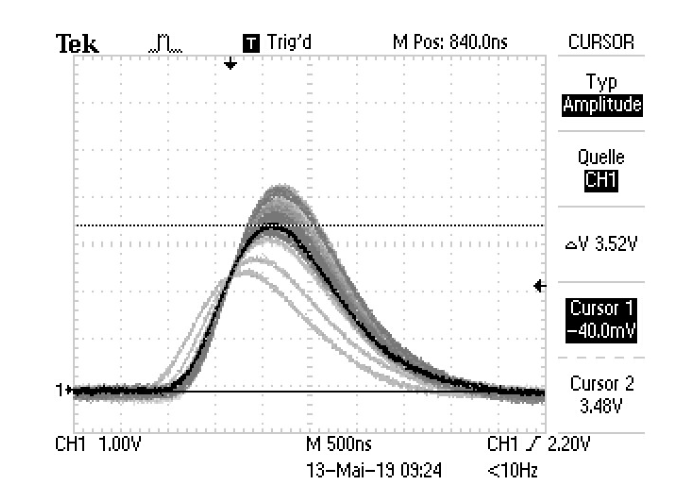
\includegraphics[height=8cm]{mitverstaerker.png}
  \caption{Impulshöhen mit Verstärker}
  \label{fig:mit}
\end{figure}

\begin{figure}[H]
  \centering
  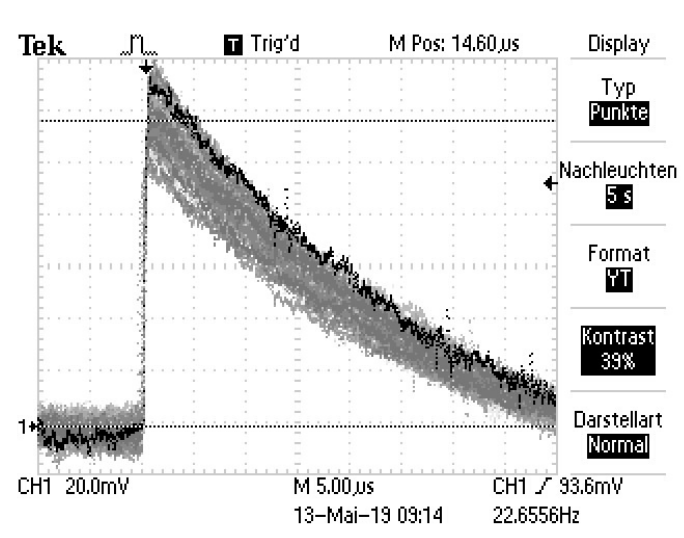
\includegraphics[height=8cm]{ohneverstaerker.png}
  \caption{Impulshöhen ohne Verstärker}
  \label{fig:ohne}
\end{figure}

Die Anstiegszeit des Signals mit Verstärker beträgt $\SI{1.3}{\micro\second}$ und die ohne Verstärker $\SI{1}{\micro\second}$.
In Abbildung \ref{fig:mit} beträgt die Impulshöhe ungefähr $\SI{3.48}{\volt}$ und in Abbildung \ref{Fig:ohne} $\SI{116}{\volt}$.



\subsection{Bestimmung der Foliendicke}
In Tabelle 1 sind die gemessenen Spannungen in Abhängigkeit des Kammerdruckes mit und ohne Goldfolie dargestellt.

\begin{table}[H]
\centering
\caption{Spannungen in Abhängigkeit des Kammerdruckes }
\sisetup{table-format=2.1}
\begin{tabular}{S S S| S S S}
  \toprule
    \multicolumn{3}{c}{Ohne Folie} & \multicolumn{3}{c}{Mit Folie} \\
    \cmidrule(lr){1-3}\cmidrule(lr){4-6}
    {$p/$mbar} & {$U/\, \symup{V}$} & {Fehler/V} & {$p$/mbar} & {$U/\, \symup{V}$} & {Fehler/V} \\
    \midrule
    0.09  & 3.66 &  0.5 & 0.12 & 2.66 & 0.5 \\
    10.0   & 3.64 &  0.5 & 10.7 & 2.50 & 0.6 \\
    20.0   & 3.52 &  0.5 & 20.5 & 2.40 & 0.6 \\
    29.8   & 3.32 &  0.5 & 32.3 & 2.30 & 0.6 \\
    40.1   & 3.32 &  0.5 & 40.8 & 2.16 & 0.6 \\
    50.2   & 3.20 &  0.6 & 50.7 & 2.00 & 0.7 \\
    60.1   & 3.12 &  0.6 & 61.2 & 1.88 & 0.6 \\
    70.5   & 3.00 &  0.5 & 72.0 & 1.74 & 0.6 \\
    80.2   & 2.96 &  0.4 & 82.3 & 1.70 & 0.7 \\
    91.8   & 2.88 &  0.5 & 92.2 & 1.58 & 0.7 \\
    100.2  & 2.80 &  0.5 & 100.7& 1.50 & 0.7 \\
    111.2  & 2.70 &  0.4 & 111.0& 1.38 & 0.8 \\
    121.2  & 2.30 &  0.5 & 122.0& 1.16 & 0.5 \\
    132.2  & 2.20 &  0.5 & 131.3& 1.04 & 0.5 \\
    141.7  & 2.10 &  0.5 & 142.9& 0.91 & 0.5 \\
    151.1  & 2.00 &  0.5 & 150.7& 0.76 & 0.3 \\
    162.2  & 1.70 &  0.5 & 160.9& 0.72 & 0.3 \\
    171.2  & 1.64 &  0.5 & 172.7& 0.68 & 0.3 \\
    181.3  & 1.58 &  0.6 & 198.0& 0.40 & 0.2 \\
    190.5  & 1.50 &  0.5 & & & \\
    200.8  & 1.30 &  0.5 & & & \\
    217.6  & 1.00 &  0.6 & & & \\
      \bottomrule
  \end{tabular}
\end{table}

In Abbildung 4 wird  die Spannung in Abhängigkeit des Druckes mit und ohne Goldfolie dargestellt. Dabei wird ein linearer
Zusammenhang zwischen Druck und Spannung angenommen:
\begin{align*}
  U = a \cdot p + b
\end{align*}

\begin{figure}[H]
  \centering
  \includegraphics[height=10cm]{build/pulsmit.pdf}
  \caption{gemessene Spannung in Abhängigkeit des Kammerdruckes.}
  \label{fig:ohne}
\end{figure}

Die Parameter der Funktion mit und ohne Folie betragen:
\begin{align*}
  &a_{\symup{mit}} = \SI{-0.0117(2)}{\volt\per\milli\bar}  \\
  &b_{\symup{mit}} = \SI{2.6(2)}{\volt}  \\
  &a_{\symup{ohne}}= \SI{-0.0123(4)}{\volt\per\milli\bar}  \\
  &b_{\symup{ohne}} = \SI{ 3.82(5)}{\volt} \\
\end{align*}

Unter der Annahme einer linearen Energieabnahme der $\alpha$-Teilchen entspricht $\Delta x$ aus Gleichung (1) der Foliendicke.
Das Verhältnis der Achsenabschnitte $b_{\symup{mit}}$ und $b_{\symup{ohne}}$ entspricht dem Verhältnis $\frac{E_{\symup{mit}}}{E_{\symup{ohne}}}$, wobei
$E_{\symup{mit}}$ und $E_{\symup{ohne}}$ die Energien bei $p=\SI{0}{\milli\bar}$ darstellen.
Für $\Delta x$ aus Gleichung (1) gilt damit:
\begin{align}
  &\Delta x = E_{\symup{ohne}} \left(1- \frac{b_{\symup{mit}}}{b_{\symup{ohne}}}\right) \frac{2 m_{\symup{0}} E_{\symup{\alpha}} (4 \pi \epsilon_0)^2}{4 \pi e^2 z_{\symup{\alpha}}  m_{\symup{\alpha}} N_{\symup{Au}} Z_{\symup{Au}} \ln{\left(\frac{4 E_{\symup{\alpha}} m_{\symup{0}}}{m_{\symup{\alpha}} I_{\symup{Au}}}\right)}} \\
  \text{mit} \:\: &\Delta E = E_{\mathrm{mit}} - E_{\mathrm{ohne}} = E_{\mathrm{ohne}} \cdot \left(1- \frac{b_{\symup{mit}}}{b_{\symup{ohne}}}\right) \\
  &E_{\symup{\alpha}} = \bar{E} = \frac{1}{2} \cdot \left(1+ \frac{b_{\symup{mit}}}{b_{\symup{ohne}}}\right)
\end{align}

Hierbei gilt für die Werte:
\begin{align*}
  &m_0 = \SI{9.109387e-31}{\kilo\gram}   \text{\cite{sample5}}\\
  &m_{\symup{\alpha}} = \SI{6.64465723e-27}{\kilo\gram} \text{\cite{sample5}}\\
  &I_{\symup{Au}} = \SI{790}{\eV} \text{\cite{sample6}}\\
  &E_{\symup{ohne}} = \SI{5.486}{\mega\eV}   \text{\cite{sample3}} \\
  &Z_{\symup{Au}} = 79 \\
  &N_{\symup{Au}} = \frac{Z \cdot \rho_{\symup{Au}}}{A \cdot u} \approx \SI{5.895e22}{\per\centi\meter\squared} \text{\cite{sample5}}\\
  &z_{\symup{\alpha}} = 2 \\
\end{align*}
%\begin{align*}
%  &m_0= \SI{9.1093897e-31}{\kilogram} \\
%  &m_{\symup{\alpha}} = \SI{6.64465723e-27}{\kilogram} \\
%  &I_{\symup{Au}} = \SI{709}{\eV} \cite{sample4}\\
%  &E_{\symup{ohne}} = \SI{5.486}{\mega\eV} \cite{sample3} \\
%  &Z_{\symup{Au}} = 79 \\
%  &N_{\symup{Au}} = \frac{Z \rho_{\symup{Au}}}{A \cdot u} = \SI{5.895e22}{\per\centi\meter\squared} \\
%  &z_{\symup{\alpha}} = 2 \\
%\end{align*}

Mit der Massenzahl $A$, der Dichte von Gold $\rho_{\symup{Au}}= \SI{19.3}{\gram\per\centi\meter\squared}$ \cite{sample7} und der atomaren Masseneinheit $u$.
Für die Foliendicke ergibt sich:
\begin{align*}
  \Delta x = \SI{3.6(6)}{\micro\meter}
\end{align*}

Der Fehler wird dabei mit der Gaußschen Fehlerfortpflanzung ermittelt:
\begin{align*}
  \sigma_{\symup{x}} = \sqrt{\left(\frac{\partial \Delta x}{\partial b_{\symup{mit}}}\sigma_{\symup{b_{\symup{mit}}}}\right)^2 + \left(\frac{\partial \Delta x}{\partial b_{\symup{ohne}}}\sigma_{\symup{b_{ohne}}}\right)^2}
\end{align*}

\begin{align*}
  \left(\frac{\partial \Delta x}{\partial b_{\symup{mit}}}\sigma_{\symup{b_{mit}}}\right)^2 = \sigma_{b_{\symup{mit}}}^{2} \left(- \frac{c \left(- \frac{b_{\symup{mit}}}{b_{\symup{ohne}}} + 1\right)}{b_{\symup{ohne}} \left(\frac{b_{\symup{mit}}}{b_{\symup{ohne}}} + 1\right) \ln^{2}{\left (d \left(\frac{b_{\symup{mit}}}{b_{\symup{ohne}}} + 1\right) \right )}} - \frac{c}{b_{\symup{ohne}} \ln{\left (d \left(\frac{b_{\symup{mit}}}{b_{\symup{ohne}}} + 1\right) \right )}}\right)^{2} \\
  \left(\frac{\partial \Delta x}{\partial b_{\symup{ohne}}}\sigma_{\symup{b_{ohne}}}\right)^2 = \sigma_{b_{\symup{ohne}}}^{2} \left(\frac{b_{\symup{mit}} c \left(- \frac{b_{\symup{mit}}}{b_{\symup{ohne}}} + 1\right)}{b_{\symup{ohne}}^{2} \left(\frac{b_{\symup{mit}}}{b_{\symup{ohne}}} + 1\right) \ln^{2}{\left (d \left(\frac{b_{\symup{mit}}}{b_{\symup{ohne}}} + 1\right) \right )}} + \frac{b_{\symup{mit}} c}{b_{\symup{ohne}}^{2} \ln{\left (d \left(\frac{b_{\symup{mit}}}{b_{\symup{ohne}}} + 1\right) \right )}}\right)^{2}
\end{align*}
Mit den Werten:
\begin{align*}
  &c =  E_{\symup{ohne}} \frac{2 m_{\symup{0}} E_{\symup{\alpha}} (4 \pi \epsilon_0)^2}{4 \pi e^2 z_{\symup{\alpha}}  m_{\symup{\alpha}} N_{\symup{Au}} Z_{\symup{Au}}} \\
  &d = \frac{2 E_{\symup{ohne}} m_{\symup{0}}}{m_{\symup{\alpha}} I_{\symup{Au}}}
\end{align*}


\subsection{Differentieller Wirkungsquerschnitt}
\label{sec:wq}
In Tabelle 2 werden die Anzahl der gemessenen Ereignisse $N$ in Abhängigkeit des Winkels $\Theta$ und der Messzeit $t$
sowie die daraus resultierende Zählrate $I$ dargestellt.


\begin{table}[H]
  \centering
  \caption{Zählrate in Abhängigkeit von Winkel und Messzeit.}
  \label{tab:Parameter}
  \begin{tabular}{c c c c}
    \toprule
    N & $\Theta/$° & $t$ /s & $I / \frac{1}{s}$\\
    \midrule
    $\SI{2219(47)}{}$ &  0 & 200 & $\SI{12.00(24)}{}$ \\
    $\SI{2120(46)}{}$ &  1 & 200 & $\SI{10.60(23)}{}$ \\
    $\SI{1748(42)}{}$ &  2 & 200 & $\SI{8.74(21)}{}$ \\
    $\SI{1477(38)}{}$ &  3 & 200 & $\SI{7.39(19)}{}$ \\
    $\SI{1684(41)}{}$ &  4 & 300 & $\SI{5.61(14)}{}$ \\
    $\SI{1317(36)}{}$ &  5 & 300 & $\SI{4.39(12)}{}$ \\
    $\SI{1218(35)}{}$ &  6 & 400 & $\SI{3.05(9)}{}$ \\
    $\SI{1199(35)}{}$ &  7 & 600 & $\SI{2.00(6)}{}$ \\
    $\SI{764(28)}{}$  &  8 & 600 & $\SI{1.27(5)}{}$ \\
    $\SI{519(23)}{}$  & 10 & 600 & $\SI{0.87(4)}{}$ \\
    $\SI{231(15)}{}$  & 12 & 600 & $\SI{0.39(3)}{}$ \\
    $\SI{83(9)}{}$    & 15 & 600 & $\SI{0.14(2)}{}$ \\
    $\SI{34(6)}{}$    & 18 & 600 & $\SI{0.06(1)}{}$ \\
    $\SI{25(5)}{}$    & 20 & 600 & $\SI{0.04(1)}{}$ \\
    \bottomrule
  \end{tabular}
\end{table}

Der differentielle Wirkungsquerschnitt wird nun aus der Gleichung
\begin{equation}
  \frac{\symup{d}\sigma}{\symup{d}\Omega} = \frac{N}{t \cdot I_0 \cdot N_\symup{Au} \cdot \Delta x \cdot \Delta \Omega}
  \label{eqn:wq}
\end{equation}
berechnet.

Dabei ist $I_0$ die Zählrate der Nullmessung ohne Folie und ergibt sich zu $I_0 =\SI{20.83(26)}{1\per\second}$.

$\Delta \Omega$ bezeichnet den pyramidenartigen Raumwinkel, der von
der effektiven Detektorfläche eingenommen wird. Um diesen zu berechnen, muss
als Erstes die effektive Detektorfläche selbst bestimmt werden. Dies geschieht
mithilfe der in Abbildung \ref{fig:skizze} gezeigten geometrischen Überlegungen.
Dabei handelt es sich um eine genauere Betrachtung des in Abbildung \ref{fig:aufbau}
gezeigten Aufbaus.

\begin{figure}[H]
  \centering
  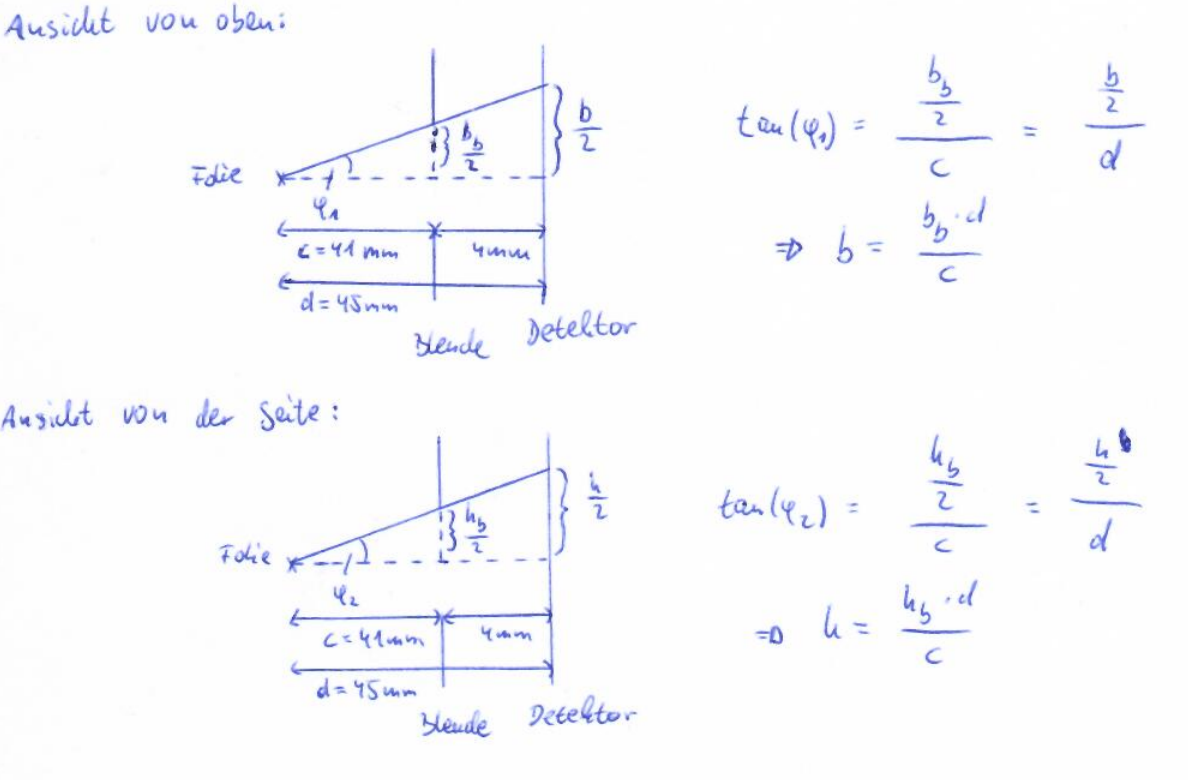
\includegraphics[height=10cm]{Skizze.PNG}
  \caption{Skizze zur Bestimmung der effektiven Detektorfläche.}
  \label{fig:skizze}
\end{figure}

Die Höhe $h$ und Breite $b$ der effektiven Detektorfläche ergeben sich also folglich
aus:
\begin{align*}
  b &= \frac{b_\symup{b} \cdot d}{c} \\
  h &= \frac{h_\symup{b} \cdot d}{c}
\end{align*}

Dabei bezeichnen $b_\symup{b}$ und $h_\symup{b}$ die Breite und Höhe der Blende.
$c$ ist der Abstand von der Folie zur Blende und $d$ ist der Abstand von der Folie
zur eigentlichen Detektoroberfläche. Diese uns bekannten Größen \cite{sample1} sind
im Folgenden noch einmal angegeben:

\begin{align*}
  b_\symup{b} = \SI{2}{\milli\meter} \\
  h_\symup{b} = \SI{10}{\milli\meter} \\
  c = \SI{41}{\milli\meter} \\
  d = \SI{41}{\milli\meter}
\end{align*}

Und daraus ergibt sich letztendlich

\begin{align*}
  b &= \SI{2.195}{\milli\meter} \\
  h &= \SI{10.976}{\milli\meter}
\end{align*}

Der Raumwinkel ergibt sich dann aus \cite{sample2}
\begin{equation}
  \Delta \Omega = 4 \cdot \arctan\left(\frac{b \cdot h}{2d \cdot \sqrt{4d^2 + b^2 + h^2}}\right) = \SI{0.0118}{sr}
\end{equation}

$N_\symup{Au}$ ist die Teilchendichte von Gold. Sie berechnet sich mit der Dichte
$\rho_\symup{Au} = \SI{19.32}{\gram\per\centi\meter^3}$ \cite{sample} und molaren Masse $M_\symup{Au} = \SI{196.97}{\gram\per\mol}$ \cite{sample}
von Gold aus
\begin{equation}
  N_\symup{Au} = N_\symup{A} \cdot \frac{\rho_\symup{Au}}{M_\symup{Au}} = 5,907 \cdot 10^{28} \, 1/\symup{m^3}
  \label{eqn:teilchendichte}
\end{equation}


$\Delta x = 2 \cdot 10^{-6} \, \symup{m}$ ist die Dicke der Folie. Daraus können dann die
differentiellen Wirkungsquerschnitte berechnet werden. Die Ergebnisse sind in Tabelle 3
in Abhängigkeit vom Winkel $\Theta$ dargestellt. Außerdem werden auch die nach
Gleichung \ref{eqn:rutherford} berechneten theoretischen Werte für die entsprechenden
Winkeln aufgeführt.


\begin{table}[H]
  \centering
  \caption{Berechnete und theoretische differentielle Wirkungsquerschnitte}
  \label{tab:Parameter}
  \begin{tabular}{c c c}
    \toprule
    $\Theta/$° & $\frac{\symup{d}\sigma}{\symup{d}\Omega}/ \mathrm{10^{-22}m^2}$ & $\frac{\symup{d}\sigma}{\symup{d}\Omega}_{\mathrm{theo}}/ \mathrm{10^{-22}m^2}$ \\
    \midrule
     0  &  $\SI{3.819(94)}{}$ & inf \\
     1  &  $\SI{3.648(91)}{}$ & $\SI{175.470}{}$ \\
     2  &  $\SI{3.008(81)}{}$ & $\SI{10.969}{}$ \\
     3  &  $\SI{2.542(73)}{}$ & $\SI{2.167}{}$ \\
     4  &  $\SI{1.932(53)}{}$ & $\SI{0.686}{}$ \\
     5  &  $\SI{1.511(46)}{}$ & $\SI{0.281}{}$ \\
     6  &  $\SI{1.048(33)}{}$ & $\SI{0.136}{}$ \\
     7  &  $\SI{0.688(22)}{}$ & $\SI{0.073}{}$\\
     8  &  $\SI{0.438(17)}{}$ & $\SI{0.043}{}$\\
    10  &  $\SI{0.298(14)}{}$ & $\SI{0.018}{}$\\
    12  &  $\SI{0.133(9)}{}$  & $\SI{0.009}{}$\\
    15  &  $\SI{0.048(5)}{}$  & $\SI{0.004}{}$\\
    18  &  $\SI{0.020(3)}{}$  & $\SI{0.002}{}$\\
    20  &  $\SI{0.014(3)}{}$  & $\SI{0.001}{}$\\
      \bottomrule
  \end{tabular}
\end{table}

Die Fehler werden hier nach der Gauß'schen Fehlerfortpflanzung bestimmt:
\begin{equation*}
  \sigma_{\frac{\symup{d}\sigma}{\symup{d}\Omega}} = \sqrt{\left(\frac{\sigma_N}{t \cdot I_0 \cdot N_\symup{Au} \cdot \Delta x \cdot \Delta \Omega}\right)^2
  + \left(\frac{N \cdot \sigma_{I_0}}{t \cdot I_0^2 \cdot N_\symup{Au} \cdot \Delta x \cdot \Delta \Omega}\right)^2}
\end{equation*}

Da es sich bei dem Versuch um ein Zählexperiment handelt, ergeben sich die Fehler der Zählraten jeweils aus der Wurzel der gezählten Ereignisse.

Die berechneten Werte und die Theoriekurve, welche sich aus Gleichung \ref{eqn:rutherford} ergibt, werden in Abbildung \ref{fig:wirkungsquerschnitt} dargestellt.

\begin{figure}[H]
  \centering
  \includegraphics{build/winkel.pdf}
  \caption{Berechneter und gemessener differentieller Wirkungsquerschnitt}
  \label{fig:wirkungsquerschnitt}
\end{figure}


\subsection{Bestimmung des Raumwinkels und der Aktivität}

Die theoretisch zu erwartende heutige Aktivität $A_{\symup{h,theo}}$ lässt sich aus dem gegebenen Wert von
$A = \SI{330}{\kilo\becquerel}$ \cite{sample1} im Oktober 1994 berechnen.

Die vergangene Zeit seit Oktober 1994 beträgt $t= (24 + \frac{8}{12})\,\symup{a}$.
Die Halbwertszeit von 241-Am beträgt $T_{1/2} = \SI{432}{a}$ \cite{sample8}, woraus sich eine
Zerfallskonstante von

$\lambda = \frac{ln(2)}{T_{1/2}} = 1,605 \cdot 10^{-3} \, \frac{1}{a}$ ergibt.
Für die heutige Aktivität ergibt sich nach dem Zefallsgesetzt somit
\begin{equation*}
  A_{\symup{h,theo}} = A \cdot exp(-\lambda t) = \SI{317190.54}{\becquerel}
\end{equation*}

Des weiteren lässt sich die heutige Aktivität $A_{\symup{h,exp}}$ aus der experimentell bestimmten
Zählrate der Nullmessung $I_0 = \SI{20.83(26)}{1\per\second}$ und dem entsprechenden Raumwinkel $\Delta \Omega_{\symup{Quelle}}$ berechnen.
$\Delta \Omega_{\symup{Quelle}}$ ist dabei der Raumwinkel um die Quelle, in welchem der Detektor bei der Nullmessung gemessen hat.
Dieser kann ganz analog zu den Überlegungen in Abbildung \ref{fig:skizze} bestimmt werden, jedoch betragen die
Abstände $c$ und $d$ hier:
\begin{align*}
  c &= \SI{97}{\milli\meter} \\
  d &= \SI{101}{\milli\meter}
\end{align*}
Grund dafür ist, dass es sich hierbei nun um die Abstände von der Quelle zur Blende
sowie von der Quelle zum Detektor handeln muss. $\Delta \Omega_{\symup{Quelle}}$ ist nämlich
der Raumwinkel um die Quelle, und nicht - wie $\Delta \Omega$ - der Raumwinkel um die Folie.
Es ergibt sich:
\begin{equation*}
  \Delta \Omega_{\symup{Quelle}} = \SI{0.0021}{sr}
\end{equation*}

Die Zählrate der Nullmessung $I_0$ und die heutige Aktivität $A_\symup{h,exp}$ müssen im gleichen
Verhältnis stehen wie der Raumwinkel $\Delta \Omega_{\symup{Quelle}}$ und der gesamte Raumwinkel:
\begin{equation*}
  \frac{A_\symup{h,exp}}{I_0} = \frac{4\pi}{\Delta \Omega_{\symup{Quelle}}}
\end{equation*}
Daraus ergbit sich
\begin{equation*}
  A_\symup{h,exp} = I_0 \cdot \frac{4\pi}{\Delta \Omega_{\symup{Quelle}}} = \SI{123.3(16)e3}{\kilo\becquerel}
\end{equation*}
Der Fehler wird dabei wieder aus der Gauß'schen Fehlerfortpflanzung bestimmt:
\begin{equation*}
  \sigma_{A_\symup{h,exp}} = \frac{4\pi}{\Delta \Omega_{\symup{Quelle}}} \cdot \sigma_{I_0}
\end{equation*}


\subsection{Untersuchung der Mehrfachstreuung}
Die Messung mit einer Goldfolie der Dicke $\Delta x = \SI{4}{\micro\meter}$ über einen
Zeitraum von $t = \SI{300}{\second}$ bei einem Winkel von $\Theta = 2 \, °$ ergibt
eine Zählrate von
\begin{equation*}
  N_\symup{4\mu m} = \SI{1033(32)}{1\per\second}
\end{equation*}
Daraus lässt sich entsprechend Gleichung \ref{eqn:wq} wieder der differentielle Wirkungsquerschnitt
berechnen. In Tabelle \ref{tab:wq} sind nun die Wirkungsquerschnitte der $\SI{2}{\micro\meter}$-Folie
und der $\SI{4}{\micro\meter}$-Folie bei dem entsprechenden Winkel von $\Theta = 2 \, °$ aufgeführt.
\begin{table}[H]
  \centering
  \caption{Differentielle Wirkungsquerschnitte der verschiedenen Goldfolien bei einem Winkel von $\Theta = 2 \, °$}
  \label{tab:wq}
  \begin{tabular}{c c}
    \toprule
    $\frac{\symup{d}\sigma}{\symup{d}\Omega}_\symup{2\mu m} /  10^{-23}\, \mathrm{m}$ & $\frac{\symup{d}\sigma}{\symup{d}\Omega}_\symup{4\mu m}/ 10^{-23}\, \mathrm{m}$ \\
    \midrule
    $\SI{30.08(81)}{}$ & $\SI{5.93(20)}{}$  \\
    \bottomrule
  \end{tabular}
\end{table}


\subsection{Untersuchung der Z-Abhängigkeit}
Die untersuchten Elemente werden mit ihrer gemessenen Zählrate $I$, der Ordnungszahl Z und der entsprechenden
Foliendicke $\Delta x$ in Tabelle \ref{tab:stoffe} aufgeführt. Des Weiteren sind die Dichte $\rho$ sowie die
molare Masse $M$ der entsprechenden Stoffe und der daraus berechenbare Term $\frac{I}{N\cdot \Delta x}$
angegeben. $N$ bezeichnet dabei die in Abschnitt \ref{sec:wq} bereits erwähnte Teilchendichte des entsprechenden Elements.
Sie berechnet sich auch hier nach Gleichung \ref{eqn:teilchendichte} für die jeweiligen Stoffe.
Der Winkel beträgt dabei $\Theta = 2 \, °$.
\begin{table}[H]
  \centering
  \caption{Spezifische Angaben und Zählraten der untersuchten Folien bei der Untersuchung der Z-Abhängigkeit \cite{sample}}
  \label{tab:stoffe}
  \begin{tabular}{c c c c c c c}
    \toprule
     & Z & $\Delta x/ \mathrm{\mu m}$ & I / $\frac{1}{\mathrm{s}}$ & $\rho/ \mathrm{\frac{g}{cm^3}}$ & M/$\mathrm{\frac{g}{mol}}$ & $\frac{I}{N\cdot \Delta x}$/$ 10^{-23}\ \mathrm{\frac{m^2}{s}}$ \\
    \midrule
    Gold & 79 & 4 & $\SI{3,44(11)}{}$ & 19,32 & 196.97 & $\SI{1.46(5)}{}$ \\
    Aluminium & 13 & 3 & $\SI{14,16(22)}{}$ & 2,70 & 26.98 & $\SI{7.83(12)}{}$ \\
    Bismut & 83 & 1 & $\SI{12,14(20)}{}$ & 9,80 & 208.98 & $\SI{42.99(71)}{}$ \\
    \bottomrule
  \end{tabular}
\end{table}

In Abbildung \ref{fig:zmessung} sind dann die berechneten Werte für $\frac{I}{N\cdot \Delta x}$
gegen die Ordnungszahl Z der jeweiligen Elemente aufgetragen.

\begin{figure}[H]
  \centering
  \includegraphics{build/z.pdf}
  \caption{$\frac{I}{N\cdot \Delta x}$ in Abhängigkeit der jeweiligen Ordnungszahl der Elemente.}
  \label{fig:zmessung}
\end{figure}

Die Fehler werden hier ganz einfach nach
\begin{equation*}
  \sigma_{\frac{I}{N\cdot \Delta x}} = \frac{\sigma_I}{N\cdot \Delta x}
\end{equation*}
berechnet.
